% ============================================================================
%  BLOQUE IV — DIAPOSITIVAS XX–XX: ESPECIFICACIÓN DEL SISTEMA
% ============================================================================
\section{Especificación del Sistema}

% ----------------------------------------------------------------------------
%  DIAPOSITIVA XX — ARQUITECTURA DE 3 CAPAS
% ----------------------------------------------------------------------------
\begin{frame}{Arquitectura de 3 Capas}
  \hypertarget{s:arquitectura}{}
  \begin{columns}[T]
    \column{0.48\textwidth}
    \footnotesize
    \textbf{Servidor de orquestación}
    \begin{itemize}
      \item Torre Ryzen 5, 16 GB RAM, Ubuntu Server headless
      \item OpenClaw Gateway (Node.js 24, puerto 18789)
      \item Ollama: qwen2.5 1.5B + mistral 7B + bge-m3
      \item Drivers Python (Tuya, BLE, FanLamp)
    \end{itemize}

    \textbf{Nodo firmware}
    \begin{itemize}
      \item ESP32 — puente BLE FanLamp
      \item \smallgray{Futuro: LIN HVAC con el mismo hardware}
    \end{itemize}

    \column{0.52\textwidth}
    \IfFileExists{\memoriaimg/fig_8_1.pdf}{%
      
\includegraphics[width=\textwidth, height=5.8cm, keepaspectratio]{\memoriaimg/fig_8_1.pdf}%
    }{%
      \fbox{\parbox{0.9\textwidth}{\centering\footnotesize [Diagrama de arquitectura]}}%
    }
  \end{columns}

  \centering
  \footnotesize
  Comunicación exclusiva sobre \texttt{192.168.1.0/24}. Ningún dato abandona el perímetro local.
\end{frame}

% ----------------------------------------------------------------------------
%  DIAPOSITIVA XX — MODEL ROUTER V2
% ----------------------------------------------------------------------------
\begin{frame}{Model Router v2: Enrutamiento en 3 Niveles}
  \hypertarget{s:router}{}
  \sloppy
  \begin{columns}[T]
    \column{0.03\textwidth}
    \column{0.63\textwidth}
    \centering
    \IfFileExists{figures/13_router.pdf}{%
      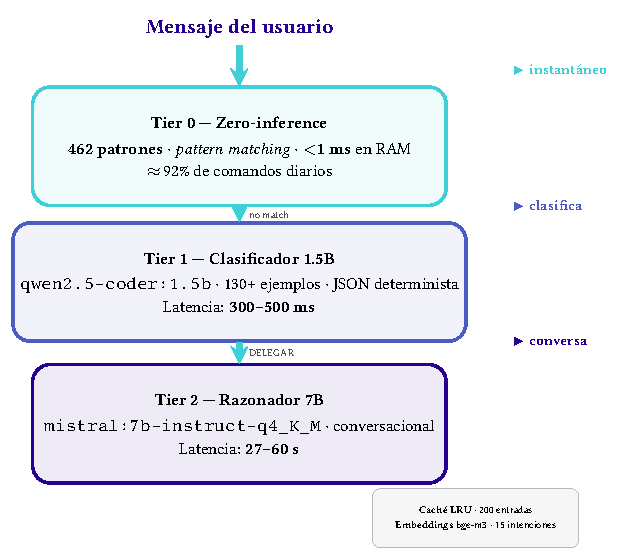
\includegraphics[width=\textwidth, height=5.8cm, keepaspectratio]{figures/13_router.pdf}%
    }{
      \textcolor{darkgray}{[Figura: flujo del Model Router v2]}
    }

    \column{0.31\textwidth}
    \centering
    \footnotesize
    \textbf{Ejemplos}\\[0.15cm]
    \renewcommand{\arraystretch}{1.1}
    \begin{tabular}{p{0.9cm}p{0.7cm}p{0.7cm}}
      \toprule
      \textbf{Com.} & \textbf{Niv.} & \textbf{Lat.} \\
      \midrule
      «vel.3» & T0 & 1,5 s \\
      «casa» & T0 & $<$1 ms \\
      «enciende» & T1 & 300 ms \\
      «buenos días» & T2 & 27--60 s \\
      \bottomrule
    \end{tabular}

    \vspace{0.3cm}
    \begin{alertblock}{Circuit Breaker}
      \footnotesize
      Si el 1.5B falla, deriva al Tier~2.
    \end{alertblock}
    \column{0.03\textwidth}
  \end{columns}
\end{frame}

% ----------------------------------------------------------------------------
%  DIAPOSITIVA XX — COMPARATIVA DE MODELOS
% ----------------------------------------------------------------------------
\begin{frame}{Selección de Modelos: Pruebas y Decisión}
  \hypertarget{s:modelos}{}
  \begin{columns}[T]
    \column{0.5\textwidth}
    \begin{block}{Proceso de evaluación}
      \footnotesize
      \textbf{Tres fases de pruebas} sobre Ryzen 5 (16 GB RAM, sin GPU)
      \begin{itemize}
        \item Corpus de 500 comandos reales
        \item Modelos probados: Qwen2.5 1.5B, Mistral 7B, Qwen3.5 4B
        \item Criterios: latencia, fiabilidad, consumo de recursos
      \end{itemize}
    \end{block}

    \begin{alertblock}{Qwen3.5: no viable en CPU}
      \footnotesize
      Versión reciente con modo \textit{thinking} forzado (no opcional).
      Resultado: 3--12 min por consulta en CPU. Diseñado para GPU.
    \end{alertblock}

    \column{0.5\textwidth}
    \begin{exampleblock}{Arquitectura seleccionada}
      \footnotesize
      \textbf{Tier 1 — Qwen2.5 1.5B} (determinista)
      \begin{itemize}
        \item 0,3--0,5 s por consulta
        \item Clasificación de comandos
      \end{itemize}
      \textbf{Tier 2 — Mistral 7B Q4} (conversacional)
      \begin{itemize}
        \item 27--60 s por consulta
        \item Razonamiento complejo
      \end{itemize}
    \end{exampleblock}

    \begin{block}{Ventaja clave}
      \footnotesize
      \textbf{Model-agnostic:} la arquitectura permite cambiar
      modelos sin modificaciones. Si un modelo futuro funciona
      mejor en CPU, se integra directamente.
    \end{block}
  \end{columns}
\end{frame}

% ----------------------------------------------------------------------------
%  DIAPOSITIVA XX — COMFORT ADVISORS
% ----------------------------------------------------------------------------
\begin{frame}{Asesores de Confort Térmico}
  \hypertarget{s:confort}{}
  \begin{columns}[T]
    \column{0.5\textwidth}
    \begin{block}{Evaluación del confort}
      \footnotesize
      El sistema evalúa continuamente:
      \begin{itemize}
        \item Condiciones interiores (temperatura, humedad)
        \item Condiciones exteriores (clima, radiación solar)
        \item Presencia de usuarios
      \end{itemize}
    \end{block}

    \column{0.5\textwidth}
    \begin{exampleblock}{Toma de decisiones}
      \footnotesize
      Basado en umbrales definidos:
      \begin{itemize}
        \item Sugiere acciones al usuario
        \item Ejecuta automáticamente si el usuario acepta
        \item Respeta siempre la decisión del usuario
      \end{itemize}
    \end{exampleblock}
  \end{columns}

  \vspace{0.5cm}
  \begin{alertblock}{Principio clave}
    \centering\footnotesize
    El sistema sugiere, el usuario decide.
  \end{alertblock}
\end{frame}

% ----------------------------------------------------------------------------
%  DIAPOSITIVA XX — AUTO-RECUPERACIÓN
% ----------------------------------------------------------------------------
\begin{frame}{Auto-Recuperación y Tolerancia a Fallos}
  \hypertarget{s:recuperacion}{}
  \centering
  \begin{columns}[T]
    \column{0.48\textwidth}
    \centering
    \IfFileExists{figures/17_recuperacion.pdf}{%
      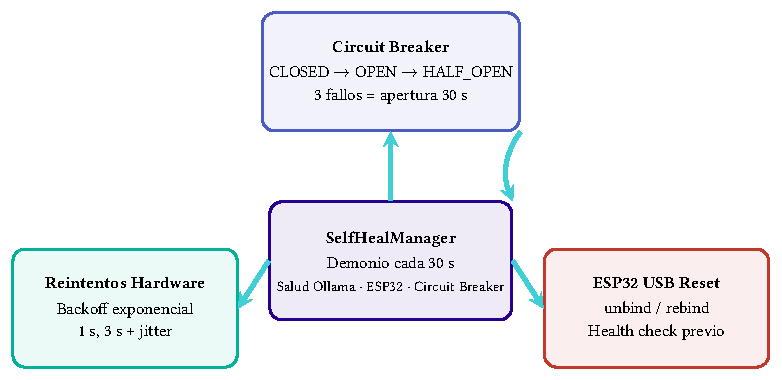
\includegraphics[width=\textwidth, height=4.5cm, keepaspectratio]{figures/17_recuperacion.pdf}%
    }{
      \textcolor{darkgray}{[Figura: ciclo de auto-recuperación]}
    }

    \column{0.48\textwidth}
    \begin{exampleblock}{Flujo de recuperación}
      \scriptsize
      \textbf{SelfHealManager} verifica cada 30\,s la salud de
      Ollama, Circuit Breaker y ESP32. Ante un fallo:
      \begin{enumerate}
        \item \textbf{Circuit Breaker} aísla el servicio
              (\texttt{CLOSED} $\to$ \texttt{OPEN})
        \item \textbf{Reintentos} con backoff + jitter (1\,s, 3\,s)
        \item Si persiste: \textbf{reset USB} del ESP32
      \end{enumerate}
      Sin intervención humana.
    \end{exampleblock}
  \end{columns}
\end{frame}
